\chapter{Reti Sequenziali, Verilog e RTL}

Gli RTL, o Register Transfer Language, permettono di descrivere cosa succede a livello di circuito fra registri. Vengono utilizzati per descrivere l'hardware. Vedremo il linguaggio \textbf{Verilog}. Gli RTL permettono di descrivere e comporre dei moduli. Il libro di testo propone il dialetto \textbf{System Verilog} che mette a disposizione due metodi per descrivere i moduli. Un metodo è il metodo \textit{constructive}, noi vedremo il metodo \textit{behavioral} dove ad esempio un Multiplexer da 2 vie 1 bit è descritto da:
\begin{lstlisting}[style={verilog}]
	z = (ic == 0 ? x : y)
\end{lstlisting}

Verilog è un linguaggio compilato. Un file System Verilog compilato produce una traccia di esecuzione e un eseguibile che simula il comportamento dei moduli. Viene detta \textbf{simulazione}.

Un programma Verilog può anche essere dato in input a un programma detto \textbf{synthetizer}, che produce una \textbf{netlist}, ovvero una lista dei componenti e dei collegamenti per realizzare il modulo fisicamente. Un altro modo per realizzare la sintesi è utilizzare un \textbf{FPGA}, o Field-programmable gate array. Un FPGA è un circuito integrato composto da una matrice di celle, e una singola cella può eseguire una funzione booleana di 3-5 ingressi con 1 uscita, implementare un bit di memoria ed effettuare routing.

Un FPGA moderno comprende, oltre a delle celle, delle righe che contengono diversi componenti come delle ALU.

\begin{figure}[H]
	\centering
	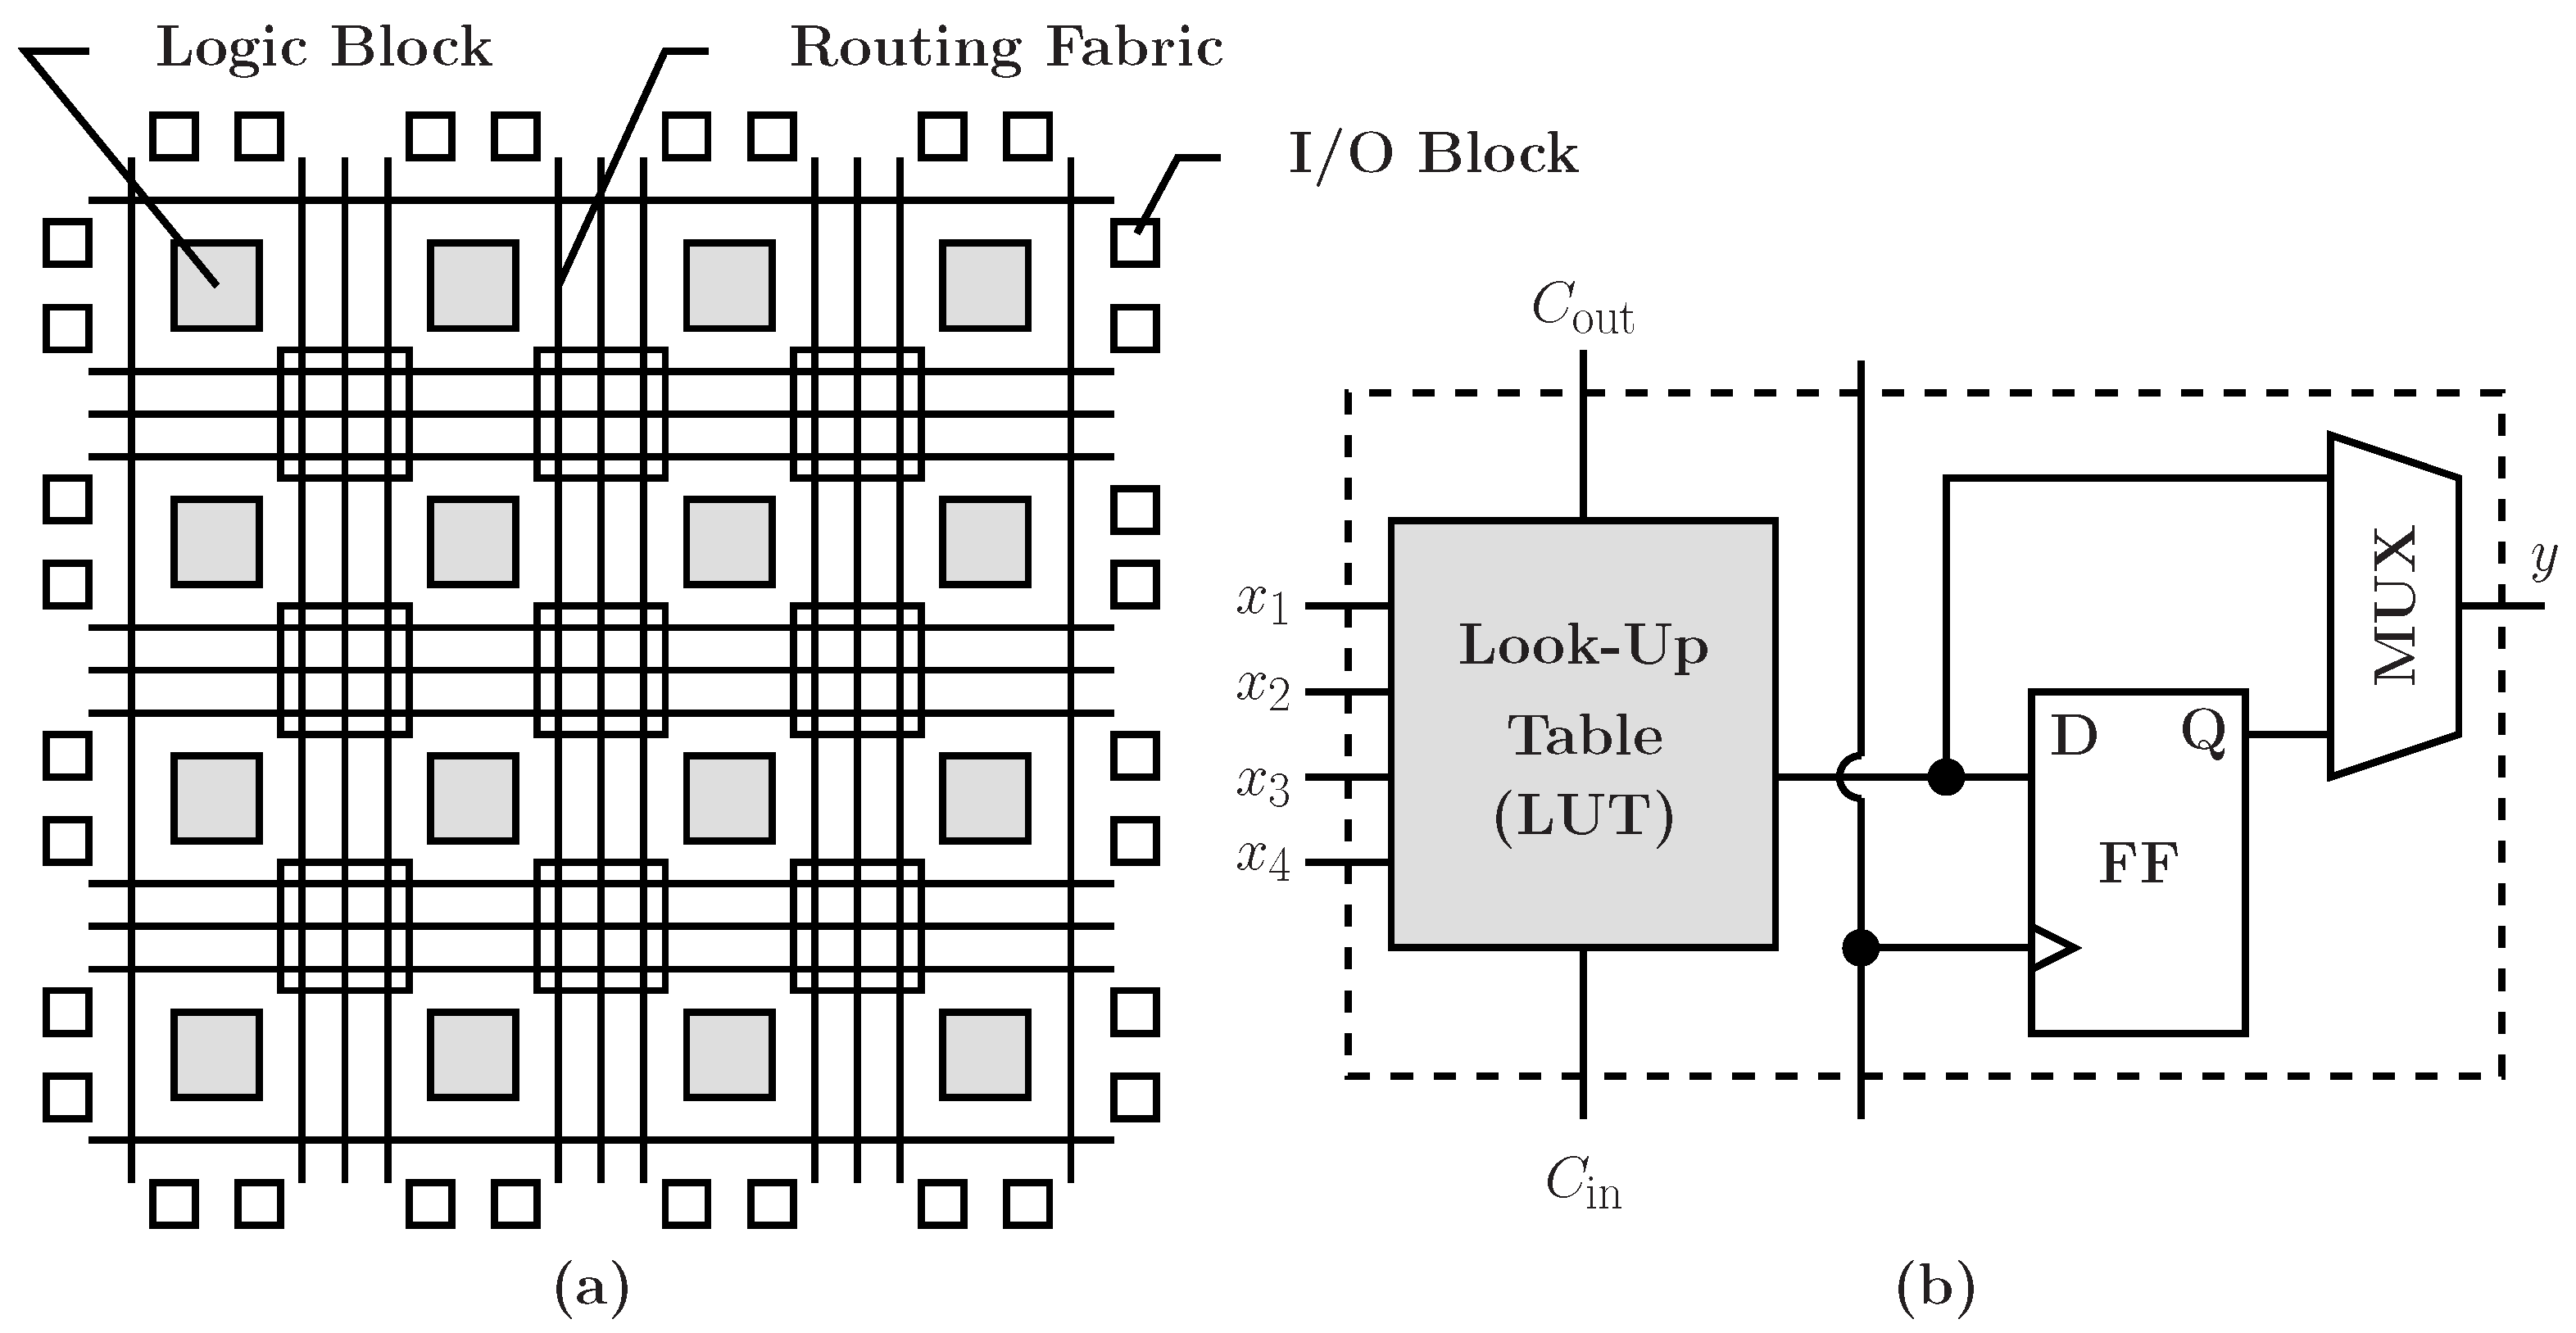
\includegraphics[]{fpga1}
	\caption{Schema FPGA}
\end{figure}

\section{Scrivere e compilare System Verilog}

Creiamo un multiplexer da due bit con System Verilog, compiliamo e visualizziamo con \textbf{GTKWave}

\includecode[verilog]{./verilog/2x1mux/mux.sv}{mux.sv}
\includecode[verilog]{./verilog/2x1mux/test_mux.sv}{test\_mux.sv}

Per compilare, eseguiamo da terminale 
\begin{lstlisting}[style={bash}]
iverilog -g2005-sv nome_sorgente.sv -o nome_eseguibile
\end{lstlisting}

Quindi, per compilare entrambi i file e caricarli in GTKWave:
\begin{lstlisting}[style={bash}]
iverilog -g2005-sv test_mux.sv mux.sv -o test_mux
# Eseguiamo la simulazione
./test_mux
# Viene creato il file provamux.vcd, carichiamolo in GTKWave
gtkwave provamux.vcd &
\end{lstlisting}

\includecode[verilog]{./verilog/2x1mux/mux4.sv}{Multiplexer da 4 vie ad 1 bit}

\includecode[verilog]{./verilog/2x1mux/muxbool.sv}{Multiplexer di variabili booleane}

\clearpage

\section{Esercizi}
\subsection{Automa che riconosce "abba"}

Realizziamo un automa di Mealy che riconosce le stringhe \textit{"abba"} da un insieme $ \{a,b,c\} $. La rete sequenziale dell'automa si realizzerà con i componenti visti in figura ~\ref{fig:mealyautomata1.tex}. Consideriamo la rappresentazione binaria dell'alfabeto con $ a = 00, b = 01, c = 11 $. Per gli stati usiamo la codifica $ S_1 = 00, S_2 = 01, S_3 = 11, S_4 = 10 $

\begin{figure}[H]
	\centering
	\caption{Automa di Mealy che riconosce "abba"}
	\begin{tikzpicture}[->,>=stealth',shorten >=1pt,auto,node distance=3.5cm]
	
	\node[state,accepting] 	(A)                    {$S_1$};
	\node[state]         	(B) [above right of=A] 	   {$S_2$};
	\node[state]         	(C) [below right of=B] 	   {$S_3$};
	\node[state]         	(D) [below right of=A] 	   {$S_4$};
	
	\path 	(A)		edge [bend left]  	node {$a/0$} 		(B)
	edge [loop left] 	node {$b,c/0$} 		(A)
	(B) 	edge [loop above] 	node {$a/0$} 		(B)
	edge [bend left] 	node {$c/0$} 		(A)
	edge [bend left]  	node {$b/0$} 		(C)
	(C)		edge [bend left]  	node {$c/0$} 		(A)
	edge [bend left]  	node {$a/0$} 		(B)
	edge [bend left]  	node {$b/0$} 		(D)
	(D)		edge [bend left]  	node {$b,c/0$} 		(A);
	\end{tikzpicture}
\end{figure}

\begin{table}[H]
	\centering
	\caption{Tabella di verità dell'output della rete sequenziale dell'automa "abba" ($ \omega $)}
	\label{tab:mealyomega2}
	\begin{tabular}{l|llll|l|}
		\cline{2-6}
		& $s_1$ & $s_2$ & $x_1$ & $x_2$ & z \\ \cline{2-6} 
		Stato $S_1$ & 0     & 0     & -     & -     & 0 \\
		Stato $S_2$ & 0     & 1     & -     & -     & 0 \\
		Stato $S_3$ & 1     & 1     & -     & -     & 0 \\
		Stato $S_4$ & 1     & 0     & 0     & 0     & 1 \\
		& 1     & 0     & 0     & 1     & 0 \\
		& 1     & 0     & 1     & 1     & 0 \\ \cline{2-6} 
	\end{tabular}
\end{table}

\begin{table}[H]
	\centering
	\caption{Tabella di verità del cambio di stato dell'automa per riconoscere "abba" ($\sigma$)}
	\label{tab:mealysigma2}
	\begin{tabular}{l|llll|ll|}
		\cline{2-7}
		& $s_1$ & $s_2$ & $x_1$ & $x_2$ & $s_1'$ & $s_2'$ \\ \cline{2-7} 
		Stato $S_1$ & 0     & 0     & 0     & 0     & 0      & 1      \\
		& 0     & 0     & 0     & 1     & 0      & 0      \\
		& 0     & 0     & 1     & 1     & 0      & 0      \\ \cline{2-7} 
		Stato $S_2$ & 0     & 1     & 0     & 0     & 0      & 1      \\
		& 0     & 1     & 0     & 1     & 1      & 1      \\
		& 0     & 1     & 1     & 1     & 0      & 0      \\ \cline{2-7} 
		Stato $S_3$ & 1     & 1     & 0     & 0     & 0      & 1      \\
		& 1     & 1     & 0     & 1     & 1      & 0      \\
		& 1     & 1     & 1     & 1     & 0      & 0      \\ \cline{2-7} 
		Stato $S_4$ & 1     & 0     & 0     & 0     & 0      & 0      \\
		& 1     & 0     & 0     & 1     & 0      & 0      \\
		& 1     & 0     & 1     & 1     & 0      & 0      \\ \cline{2-7} 
	\end{tabular}
\end{table}

Avremo che la formula booleana sarà per il primo e secondo bit di stato:
\[ s_1' = \overbar{s_1}s_2\overbar{x_1}x_2 + s_1s_2\overbar{x_1}x_2 = s_2\overbar{x_1}x_2 \]. 
\[ s_2' = \overbar{s_1s_2}+ \overbar{s_1}s_2\overbar{x_1} + s_2\overbar{x_2}\]

Nella componente \verb|sigma| in Verilog avremo l'assegnamento ad un nuovo stato \verb|news|:

\begin{lstlisting}[style={verilog}]
assign
	news[1] = s[2] & ~x[1] & x[2];

assign    
	news[2] = ~s[1] & ~x[1] & ~x[2] 
		| s[2] & ~x[1] & ~x[2] 
		| ~s[1] & s[2] & ~x[1];
\end{lstlisting}

La formula per l'uscita sarà $ z = s_1\overbar{s_2x_1x_2} $. La componente \verb|omega| effettuerà l'assegnamento 

\begin{lstlisting}[style={verilog}]
assign
	z = s[1] & ~s[2] & ~x[1] & ~x[2];
\end{lstlisting}



 Ci rimane da definire il registro da 2 bit per definire tutta la rete sequenziale. Abbiamo supposto che la rete sequenziale funzioni ricevendo un segnale di clock ad intervalli regolari.
La rete di output $ \omega $ è definita utilizzando soltanto AND ed impiegherà $ \Delta t $ per eseguire l'operazione. La funzione di cambio di stato $ \sigma $ è definita invece con 1 AND e 1 OR ed impiegherà $ 2\Delta t $ per l'operazione.
Il ciclo di clock dev'essere almeno $ \tau = \delta + \max\{t_{\sigma}, t_{\omega}\} $ dove $ \delta $ è la durata del segnale HIGH nel clock.

Abbiamo 3 moduli. Uno per il registro, uno per il modulo $ \omega $ e uno per il modulo $ \sigma $. Scriviamolo in Verilog.

\paragraph{Note sulla sintassi e semantica Verilog}

La sintassi \verb|[a:b]| denota un array indicizzato dal numero \verb|a| al numero \verb|b|. Utilizziamo gli array per rappresentare valori a più bit. In questo caso, il registro è generalizzato per un parametro \verb|N| e può ad esempio essere inizializzato con \verb|registro #(4) nome(...) | dove 4 è il parametro \verb|N| e corrisponde al numero di bit del registro.

La negazione con \verb|!| nega un singolo valore, mentre la notazione \verb|~| viene detta negazione \textit{bit wise} e nega tutti i valori di una sequenza di bit.

Normalmente, in un blocco \verb|assign| assegno un valore ad una variabile booleana istantaneamente. Posso invece aggiungere un delay inserendo \verb|#x| di fronte all'identificatore della variabile, dove \verb|x| è un numero. Ad esempio:
\begin{lstlisting}[style={verilog}]
assign 
	#1 z = (ic == 0 ? x : y)
\end{lstlisting}

\includecode[verilog]{./verilog/abba/Registro/reg.v}{Registro a N bit}
\includecode[verilog]{./verilog/abba/Mealy/sigma.v}{Modulo di $ \sigma $ o funzione di cambio di stato}
\includecode[verilog]{./verilog/abba/Mealy/omega.v}{Modulo di $ \omega $}
\includecode[verilog]{./verilog/abba/Mealy/m1.v}{Modulo della rete sequenziale}
\includecode[verilog]{./verilog/abba/MealyInSync/m1.v}{Modulo della rete sequenziale (con Sincronizzazione)}
\includecode[verilog]{./verilog/abba/Mealy/test-m1.v}{Modulo di test della rete sequenziale}
\includecode[makefile]{./verilog/abba/Mealy/makefile}{Makefile}


Per sincronizzare il modulo della rete sequenziale dell'automa di Mealy mettiamo un registro di fra l'input \verb|x| e le reti sequenziali \verb|sigma| e \verb|omega|.

\begin{figure}[!htb]
	\centering 
	\caption{Diagramma dei tempi della Rete Sequenziale dell'automa di Mealy per riconoscere "abba" \textbf{senza sincronizzazione}}
	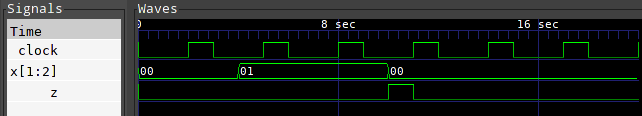
\includegraphics[width=\textwidth]{mealyabbanosync.png}
\end{figure}

\begin{figure}[!htb]
	\centering 
	\caption{Diagramma dei tempi della Rete Sequenziale dell'automa di Mealy per riconoscere "abba" \textbf{con sincronizzazione}}
	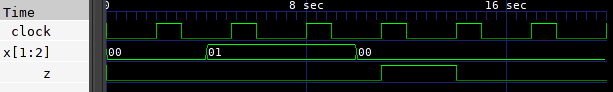
\includegraphics[width=\textwidth]{mealyabbainsync.png}
\end{figure}

\FloatBarrier

\subsection{Automa di Moore per riconoscere "abba"}
Vediamo adesso un automa di Moore per riconoscere la stringa \textit{"abba"} nell'alfabeto $ \{a,b,c\} $. La differenza sta nel fatto che i singoli nodi non hanno accesso all'input $ x $. Teniamo nota che la differenza fra un automa di Mealy di un automa di Moore, consiste che nell'automa di Moore la funzione $ \omega $ non accetta riceve l'input

\begin{figure}[H]
	\centering
	\caption{Automa di Moore che riconosce "abba"}
	\begin{tikzpicture}[->,>=stealth',shorten >=1pt,auto,node distance=3.5cm]
	
	\node[state,initial] 	(A)                    {$\dfrac{S_1}{0}$};
	\node[state]         	(B) [right of=A] 	   {$\dfrac{S_2}{0}$};
	\node[state]         	(C) [below of=A] 	   {$\dfrac{S_3}{0}$};
	\node[state]         	(D) [below of=B] 	   {$\dfrac{S_4}{0}$};
	\node[state,accepting]  (E) [above right of=D] 	   {$\dfrac{S_5}{1}$};
	
	\path 	(A)		edge [bend left=60]  				node {$a$} 		(B)
					edge [loop above] 					node {$b,c$} 	(A)
			(B) 	edge [loop above] 					node {$a$} 		(B)
					edge [] 							node {$c$} 		(A)
					edge [bend left=20]  				node {$b$} 		(C)
			(C)		edge []  							node {$c$} 		(A)
					edge [bend left=20]  				node {$a$} 		(B)
					edge []  							node {$b$} 		(D)
			(D)		edge [bend left=90,looseness=2]		node {$b,c$} 	(A)
					edge []								node {$a$}		(E)
			(E)		edge [bend right=90,looseness=1.8]  	node {$b,c$} 	(A)
					edge []	node {$a$}		(B);
	\end{tikzpicture}
\end{figure}

\diagram{mooreautomata1.tex}{Rete Sequenziale dell'automa di Moore per riconoscere \textit{"abba"}}

\includecode[verilog]{./verilog/abba/Moore/mo-sigma.v}{Modulo di $ \sigma $ o funzione di cambio di stato (Moore)}
\includecode[verilog]{./verilog/abba/Moore/mo-omega.v}{Modulo di $ \omega $ (Moore)}
\includecode[verilog]{./verilog/abba/Moore/moore.v}{Modulo della rete sequenziale (Moore)}
\includecode[verilog]{./verilog/abba/Moore/test-m1.v}{Modulo di test della rete sequenziale (Moore)}

\FloatBarrier

\subsection{Mealy con Delay $ \equiv $ Moore}

Vedremo come in termini di esecuzione, introducendo dei delay nell'automa di Mealy otteniamo un comportamento analogo all'automa di Moore.

\includecode[verilog]{./verilog/abba/MealyConDelay/sigma-delay.v}{Modulo di $ \sigma $ o funzione di cambio di stato (Mealy con Delay)}
\includecode[verilog]{./verilog/abba/MealyConDelay/omega-delay.v}{Modulo di $ \omega $ (Mealy con Delay)}
\includecode[verilog]{./verilog/abba/MealyConDelay/reg-delay.v}{Registro a N bit con delay}
\includecode[verilog]{./verilog/abba/MealyConDelay/m1-delay.v}{Modulo della rete sequenziale (Mealy con Delay)}
\includecode[verilog]{./verilog/abba/MealyConDelay/test-m1-delay.v}{Modulo di test della rete sequenziale (Mealy con Delay)}


\FloatBarrier

\section{Componenti per il Calcolo}

Nel capitolo precedente abbiamo visto gli \textbf{adder}, che accettano due bit e restituiscono bit sommato e riporto, e abbiamo visto i \textbf{full adder}, che accettano in input anche un riporto per poter essere composti a cascata. Tutti i tempi di stabilizzazione dei full adder si sommano l'uno con l'altro. Ciò è chiaramente un problema perché se dobbiamo sommare due numeri da 32 bit dobbiamo aspettare la stabilizzazione di 32 sommatori. Oppure, sommando due numeri da 4 bit avremo $ 4 \cdot 2 \Delta t = 8 \Delta t $
\diagram{sum.tex}{Sommatori di due numeri}
Per ovviare al problema possiamo realizzare $ n + 1 $ tabelle di verità (ognuna per ogni bit di input, più il riporto che indica se è avvenuto un overflow). Le tabelle di verità avranno $ 2^{2n} $ righe. Ad esempio, per sommare due numeri da 4 bit avremo 1 livello AND e 3 livelli OR perché usiamo porte che accettano al massimo 8 entrate. Ciò impiegherà (per numeri da 4 bit) $ 4 \Delta t $ a differenza della somma con Full Adder a cascata che impiega $ 8 \Delta t $.

Se volessi sommare numeri da 8 bit, la situazione varia leggermente. Servono 2 livelli di AND, e per esprimere la tabella di verità servono al minimo $ 2^{15} $ righe. I livelli di OR saranno quindi $ \ceil{\dfrac{\log_2 2^{15}}{log_2 2^3}} =  \ceil{\dfrac{15}{3}} $.

% TODO high e low sommatore da 8 bit con due FA da 4 bit per rispettare il limite delle porte

\paragraph{ALU con sottrattore}

Possiamo realizzare la sottrazione in questo modo (funziona anche per i numeri negativi se utilizziamo il complemento a due):
\begin{enumerate}
	\item Vogliamo sottrarre un numero $ B = 4 \equiv 00000100$ ad un altro numero $ A = 12 \equiv 00001100 $: $ A - B = 8 \equiv 00001000 $
	\item Invertiamo B e aggiungiamo 1: $ (\overbar{B} + 1) \equiv 11111100 $
	\item Otteniamo che $ A - B \equiv A + (\overbar{B} + 1) \equiv 000001000 $ (non va considerato l'overflow)	
\end{enumerate}

Un possibile (ma errato) circuito che realizza sottrazione e addizione può essere il seguente:

\diagram{addsubtract1}{ALU per addizione e sottrazione}

Si può semplificare molto il circuito utilizzando un ALU per la somma che accetta un riporto iniziale come i full adder a cascata.

\diagram{addsubtract2}{ALU per addizione e sottrazione semplificata}

\paragraph{Uscite aggiuntive delle ALU o flag}

Le ALU, oltre all'uscita del risultato possono avere delle uscite aggiuntive, dette \textbf{flag}. I flag più comuni sono il flag \textbf{Z}ero, il flag \textbf{N}egative ed il flag \textbf{C}arry.

Il flag \textbf{Z} (Zero) è 1 se tutti i bit del risultato sono 0. Ovvero $ Z = \forall i \>.\> (\text{out}_i == 0) $. Si può realizzare inserendo nella alu un gate NOR che riceve in entrata tutti i bit dell'output.

Il flag \textbf{N} (Negative) è semplicemente il bit più significativo (a sinistra) se utilizziamo la notazione a complemento a due.

Il flag \textbf{C} (Carry) è usato per indicare se un riporto è stato generato nell'output dal bit più significativo. Permette di realizzare ALU composte da altre ALU, con dimensioni di parole in bit maggiori di quella della singola unità aritmetica. Il bit di carry della ALU che calcola la sezione LOW della parola viene inserito come riporto iniziale della ALU che calcola la parte HIGH della parola.


\paragraph{Moltiplicatore}

\begin{table}[H]
	\begin{tabular}{llllllll}
		&          &          &          & 1 & 0 & 1 & 1 \\
		&          &          & $\times$ & 1 & 1 & 0 & 1 \\ \cline{5-8} 
		&          &          & $^{(1)}$ & 1 & 0 & 1 & 1 \\
		&          & $^{(1)}$ & 0        & 0 & 0 & 0 &   \\
		& $^{(1)}$ & 1        & 0        & 1 & 1 &   &   \\
		& 1        & 0        & 1        & 1 &   &   &   \\ \cline{2-8} 
		1 & 0        & 0        & 0        & 1 & 1 & 1 & 1
	\end{tabular}
	\caption{Moltiplicazione binaria $11 \times 13 = 143$}
	\label{tab:binmult}
\end{table}


La moltiplicazione binaria avviene in maniera analoga alla normale moltiplicazione in colonna. Ciò ci permette di visualizzare rapidamente un possibile circuito realizzato da moltiplicazione e somma dei risultati. È facile osservare che la moltiplicazione fra due singole cifre binarie è banalmente il gate AND. Per realizzare un circuito moltiplicatore sarà necessario quindi una "matrice" di gate AND e dei sommatori in fondo. Per l'ultimo ed il primo bit della somma saranno necessari solamente degli Half Adder, perché non accettano un riporto in input.


\centerfig{0.75}{4bitbinmult}{Circuito di un moltiplicatore interno ad una ALU di due numeri da 4 bit $ A $ e $ B $}

\includecode[verilog]{./verilog/mul4bit/notiming/ha.v}{Half Adder in Verilog}
\includecode[verilog]{./verilog/mul4bit/notiming/fa.v}{Full Adder in Verilog}
\includecode[verilog]{./verilog/mul4bit/notiming/mul4bit.v}{mul4bit.v}

